\documentclass[12pt,reqno]{article}
\usepackage{amsthm, amsmath, amsfonts, amssymb, amscd, mathtools, youngtab, euscript, mathrsfs, verbatim, enumerate, multicol, multirow, bbding, color, babel, esint, geometry, tikz, tikz-cd, tikz-3dplot, array, enumitem, hyperref, thm-restate, thmtools, datetime, graphicx, tensor, braket, slashed, standalone, pgfplots, ytableau, subfigure, wrapfig, dsfont, setspace, wasysym, pifont, float, rotating, adjustbox, pict2e,array}
\usepackage{amsmath}
\usepackage[utf8]{inputenc}
\usetikzlibrary{arrows, positioning, decorations.pathmorphing, decorations.pathreplacing, decorations.markings, matrix, patterns}
\tikzset{big arrow/.style={
    decoration={markings,mark=at position 1 with {\arrow[scale=1.5,#1]{>}}},
    postaction={decorate},
    shorten >=0.4pt},
  big arrow/.default=black}

\begin{document}

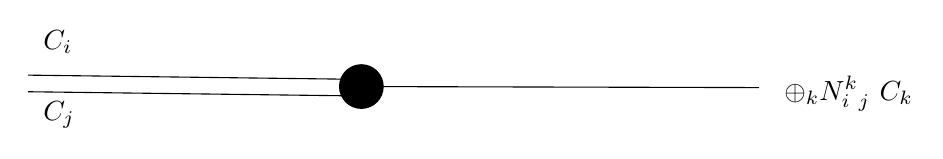
\begin{tikzpicture}[x=0.75pt,y=0.75pt,yscale=-1,xscale=1]

\draw    (129,76) -- (286,78) ;
\draw    (129,84) -- (286,86) ;
\draw  [fill={rgb, 255:red, 0; green, 0; blue, 0 }  ,fill opacity=1 ] (279,81.5) .. controls (279,75.7) and (283.7,71) .. (289.5,71) .. controls (295.3,71) and (300,75.7) .. (300,81.5) .. controls (300,87.3) and (295.3,92) .. (289.5,92) .. controls (283.7,92) and (279,87.3) .. (279,81.5) -- cycle ;
\draw    (289.5,81.5) -- (481,82) ;

% Text Node
\draw (135,53.4) node [anchor=north west][inner sep=0.75pt]    {$C_{i}$};
% Text Node
\draw (135,87.4) node [anchor=north west][inner sep=0.75pt]    {$C_{j}$};
% Text Node
\draw (492,75.4) node [anchor=north west][inner sep=0.75pt]    {$\oplus _{k} N_{i\ j}^{k} \ C_{k}$};


\end{tikzpicture}

\end{document}